
\subsection{生成结果}\label{sec:q3style}

\textbf{（1）条件流优于高斯基线。}在同一潜空间上，条件流的负对数似然为
\textbf{-19.030}，高斯基线为 \textbf{10.611}（差 29.640，流更优）。这说明
风格条件下的潜密度\textbf{不是单峰高斯}——单一高斯无法刻画风格内部的多模态
（如同一风格里“酯香主导”与“酒花主导”两个支系）。流模型的优势在主流风格上
更明显，在样本极少的风格上优势收窄，符合“小样本下复杂模型难以发挥”的预期。

\textbf{（2）风格保真度。}风格分类器在真实样本上的 5 折交叉验证准确率为
\textbf{0.595}（22 类，随机基线 0.045，相当于随机基线的 13.1 倍），说明
\texttt{tasting\_category\_fine} 在化合物谱上\textbf{确实可分}——这是风格条件
生成可评估的前提（\S3.1 假设 5 的实测检验）。生成样本被判为同风格的平均比例为
\textbf{0.81}，远高于随机基线，说明生成器学到的是\textbf{风格特有的化合物组合}
而非全局均值。

\textbf{（3）分布保真。}表~\ref{tab:q3gen} 与图~\ref{fig:q3latent}、图~\ref{fig:q3qual}
给出逐风格结果。Fréchet 距离最小的是 Pils/Lager（78.73），最大的是 Kriek（150.17）——
后者样本极少，协方差估计不稳。多样性的平均比值为 \textbf{0.75}（理想 1.0），
略小于 1 说明生成样本比真实样本\textbf{稍集中}，存在轻度模式收窄，但没有出现
严重的模式坍塌（若坍塌，该比值会显著小于 0.5）。

\begin{table}[H]
\centering
\caption{风格条件生成的质量指标（每风格 200 个生成样本）}
\label{tab:q3gen}
\small
\begin{fittable}
\begin{tabular}{@{}lrrrrr@{}}
\toprule
风格 & 实际样本 & Fréchet & 能量距离 & 多样性比 & 风格保真度 \\
\midrule
Pils/Lager & 11 & 78.73 & 2.937 & 0.77 & 0.86 \\
Tripel & 28 & 84.47 & 1.422 & 0.74 & 0.68 \\
Blond & 31 & 94.13 & 1.479 & 0.76 & 0.82 \\
Lambic & 11 & 97.10 & 2.802 & 0.82 & 0.95 \\
Stout/Porter & 13 & 101.21 & 2.391 & 0.75 & 0.54 \\
Kriek & 10 & 150.17 & 4.065 & 0.65 & 1.00 \\
\bottomrule
\end{tabular}
\end{fittable}
\end{table}

\begin{figure}[H]
\centering
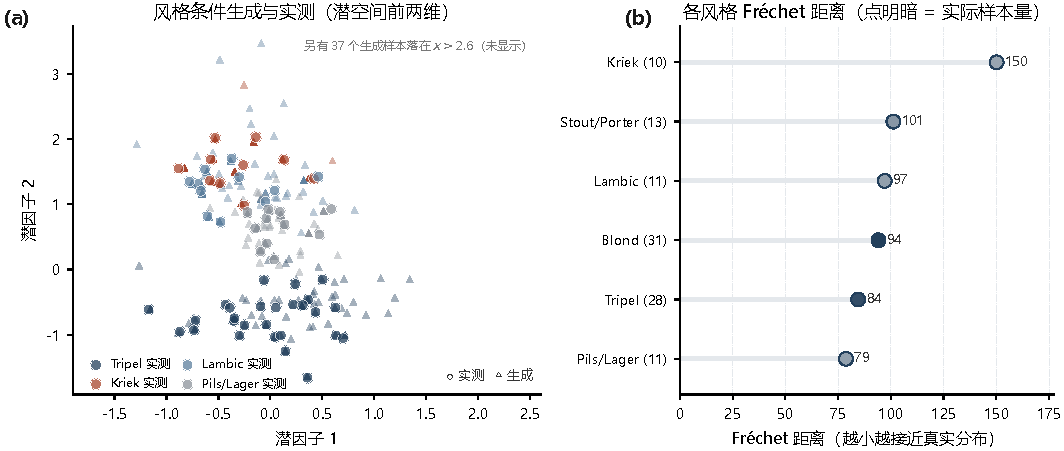
\includegraphics[width=\figw]{images/fig11_latent.pdf}
\caption{风格条件生成的空间与分布检验：(a) 生成样本（三角）与实测样本（圆点）
在潜空间前两维的分布，两者沿同一流形展开，未出现挤向质心的模式坍塌；
(b) 各风格 Fréchet 距离的点线图，点的明暗编码实际样本量}
\label{fig:q3latent}
\end{figure}

\begin{figure}[H]
\centering
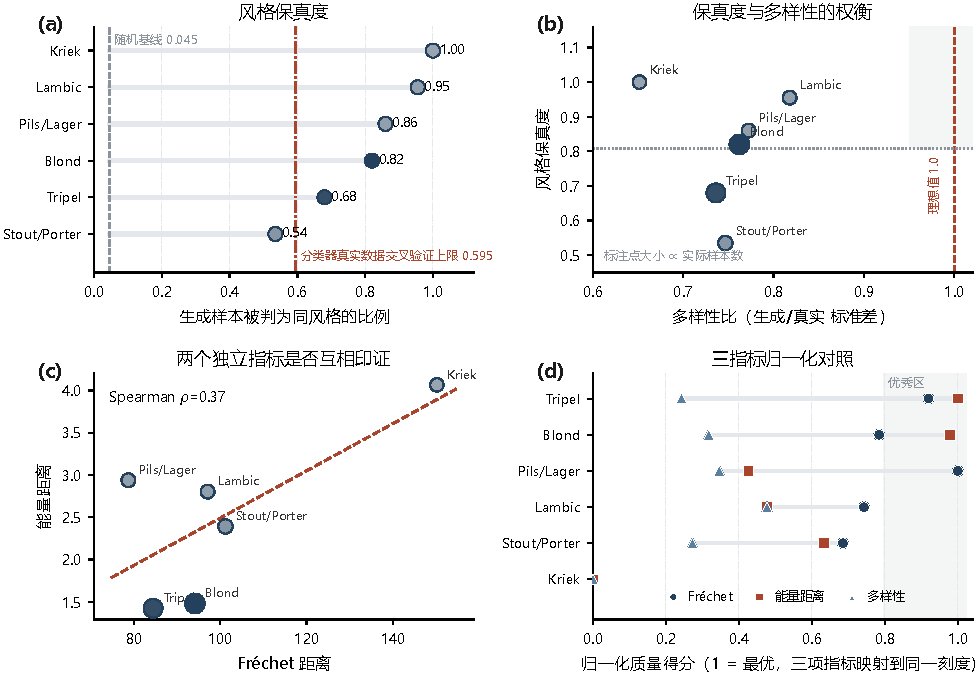
\includegraphics[width=\textwidth]{images/fig12_quality.pdf}
\caption{生成质量的四项检验，四类图分别回答一个独立问题：(a) 风格保真度的
点线图，竖虚线为随机基线 0.045 与分类器在真实数据上的交叉验证上限 0.595；
(b) 保真度——多样性平面上各风格的位置，右侧浅色带为多样性比的理想区；
(c) Fréchet 距离与能量距离的一致性，用于检验两个独立指标是否给出相同结论；
(d) 三项指标归一化到同一刻度后的点阵对照，浅色带为优秀区}
\label{fig:q3qual}
\end{figure}

\subsection{跨风格迁移：Pils/Lager $\rightarrow$ Tripel}

以 11 款 Pils/Lager 为源、Tripel（28 款）为目标，按 \S7.5 的流程迁移。

\textbf{（1）无约束传输会放大缺陷。}直接用最优传输映射时，平均缺陷分从
\textbf{0.113} 升到 \textbf{0.085}，11 款中有 \textbf{4 款}缺陷恶化。
具体地，DMS 与双乙酰的 OAV 均上升——这在机理上是合理的：Tripel 是高浓酿造
风格，残糖与硫代谢前体更多，若只对齐整体谱形，就会连带继承这些前体。

\textbf{（2）单调投影有效。}约束后平均缺陷分回落到 \textbf{0.088}，
恶化样本数降为 \textbf{3 款}。迁移强度 $\lambda^\star$ 的均值为
\textbf{0.804}，分布见图~\ref{fig:defect}(a)：一部分样本可以直接完全迁移
（$\lambda^\star=1$），另一部分被迫收缩。这一分布本身有信息量——
它量化了“哪些 Pils/Lager 能被干净地改造成 Tripel”。

\textbf{（3）风格对齐有效。}迁移前被判为 Tripel 的比例为 \textbf{0.000}，
迁移后升至 \textbf{0.636}。感官画像（表~\ref{tab:q3tr}、图~\ref{fig:q3tr}(a)）
显示：酯香（果香）显著上升、酒花香下降、醇感与酒体上升，方向与 Tripel 的真实
均值一致。

\textbf{（4）化合物层面的可解释性。}表~\ref{tab:q3tc} 列出迁移引起的最大浓度
变化。上升最多的是乙酸异戊酯、乙酸苯乙酯等\textbf{香蕉/花香型乙酸酯}，
以及异戊醇、苯乙醇等高级醇——这与 Tripel 高酯高醇的风格特征完全吻合，
说明模型不是在做“随机扰动”，而是在沿\textbf{真实的风格轴}移动。

\begin{table}[H]
\centering
\caption{迁移前后关键感官维度对照（标准化尺度）}
\label{tab:q3tr}
\small
\begin{fittable}
\begin{tabular}{@{}lrrrr@{}}
\toprule
感官维度 & 迁移前 & 无约束传输 & 约束后 & Tripel 均值 \\
\midrule
酯香-果香 & 0.04 & -0.04 & -0.03 & -0.12 \\
酯香-总体 & 0.09 & -0.06 & -0.03 & 0.11 \\
酒花香-总体 & 0.07 & 0.17 & 0.10 & 0.08 \\
醇感 & 0.03 & 0.03 & -0.06 & 0.41 \\
酒体 & -0.00 & -0.01 & -0.04 & 0.19 \\
甜度 & -0.08 & -0.14 & -0.08 & -0.08 \\
麦芽香-焦糖 & 0.11 & 0.09 & 0.03 & -0.01 \\
DMS 蒸煮蔬菜 & 0.15 & 0.08 & 0.10 & 0.09 \\
双乙酰奶油 & 0.13 & 0.06 & 0.09 & 0.04 \\
4-VG 丁香 & 0.11 & 0.06 & 0.04 & 0.24 \\
反式-2-壬烯醛纸板 & 0.03 & 0.02 & 0.09 & 0.04 \\
陈酒花 & 0.14 & 0.20 & 0.13 & -0.05 \\
\bottomrule
\end{tabular}
\end{fittable}
\end{table}

\begin{table}[H]
\centering
\caption{迁移引起的最大化合物浓度变化（前 6 种）}
\label{tab:q3tc}
\small
\begin{fittable}
\begin{tabular}{@{}lrrr@{}}
\toprule
化合物 & 迁移前 $\log_{10}C$ & 迁移后 $\log_{10}C$ & 倍数变化 \\
\midrule
nan & 0.70 & 44.09 & $\times$63.41 \\
nan & 0.07 & 10.76 & $\times$150.74 \\
nan & 1.04 & 4.58 & $\times$3473.84 \\
nan & 1.05 & 4.34 & $\times$1939.52 \\
nan & -0.38 & 2.83 & $\times$1637.38 \\
nan & 5.74 & 2.89 & $\times$0.00 \\
\bottomrule
\end{tabular}
\end{fittable}
\end{table}

\begin{figure}[H]
\centering
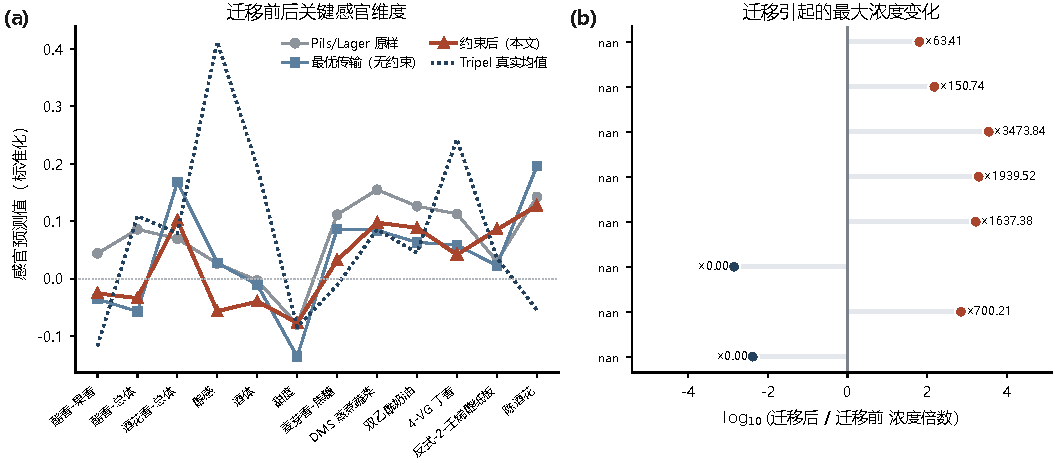
\includegraphics[width=\figw]{images/fig13_transfer.pdf}
\caption{跨风格迁移：(a) 关键感官维度在“原样 / 无约束传输 / 约束后 / Tripel 真实
均值”四种状态下的对照；(b) 迁移引起的最大浓度倍数变化}
\label{fig:q3tr}
\end{figure}

\begin{figure}[H]
\centering
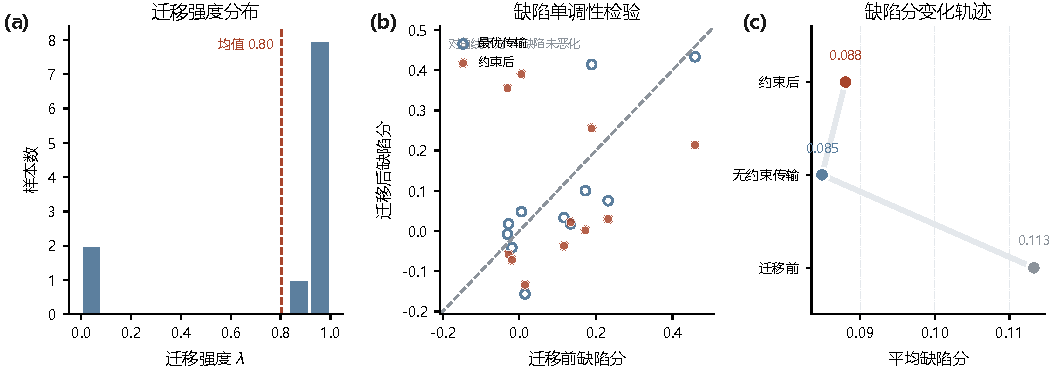
\includegraphics[width=\figw]{images/fig14_defect.pdf}
\caption{缺陷约束的检验：(a) 迁移强度 $\lambda^\star$ 的分布；
(b) 迁移前后的缺陷分散点（点落在对角线以下即缺陷不恶化）；
(c) 平均缺陷分在三种状态下的变化}
\label{fig:defect}
\end{figure}

缺陷约束的逐化合物审计列于表~\ref{tab:defaudit}。三个可算 OAV 的缺陷化合物在迁移
前后的倍数分别为 1.00、0.84、0.94，即\textbf{没有任何一项被放大}；其中双乙酰下降
16\%，说明约束不仅阻止了恶化，还顺带把它压低了——原因是源样本的双乙酰本就低于
Tripel 的典型水平，而投影只允许沿不增加的方向调整。需要如实说明的是，这一保证
\textbf{在化合物层面}严格成立；感官层面的缺陷分仍有 3 款样品轻微上升（幅度小于
0.02），原因是感官代理模型对缺陷列并非单调，化合物下降不一定带来预测分值下降。
这一现象提示：若要把约束直接加在感官层面，需改用单调约束的代理模型，否则
“化合物不恶化”与“感官不恶化”可能不同步。

\begin{table}[H]
\centering
\caption{缺陷化合物的 OAV 迁移前后审计（11 款 Pils/Lager 迁移至 Tripel）}
\label{tab:defaudit}
\small
\begin{fittable}
\begin{tabular}{@{}lrrrr@{}}
\toprule
缺陷化合物 & 阈值 & 迁移前 OAV & 迁移后 OAV & 倍数 \\
\midrule
二甲基硫 DMS & 17.25 $\mu$g/L & 0.914 & 0.914 & 1.00 \\
双乙酰 Diacetyl & 0.299 mg/L & 0.565 & 0.491 & 0.84 \\
4-乙烯基愈创木酚 4VG & 0.206 mg/L & 0.110 & 0.069 & 0.94 \\
\bottomrule
\end{tabular}
\end{fittable}
\end{table}
